\chapter{Research}\label{research} \todo{Change Title}
This chapter, or series of chapters, delves into all technical details that are required to \emph{prove} your scientific hypothesis.
Please do not call this chapter or these chapters \emph{Research} as that name is not descriptive.
It should be sufficiently detailed and precise in order for any fellow computing scientist student to be able to \emph{repeat} your research and therewith establish the same results \slash{} conclusions that you have obtained.
Please note that, in order to improve readability of your thesis, you can put a part of this information also in one or more appendices (see Appendix~\ref{appendix}).


\section{Pipeline Setup}
In order to correctly verify the summary given by the LLM model, we have to create a pipeline that sources the needed context. As seen in Chapter \ref{Newsletter}, the newsletter contains a one-sentence summary. Before we can validatie whether this is true or not, we need to extract all context. This is done by loading the URL using a headless browser, where we scrape the Dutch text. This then gets parsed and cleaned, and sent to the validator. Meanwhile, the summary gets chopped into atomic claims, who then can be validated. A diagram can be found in figure \ref{fig:pipeline_flowchart}. 
\begin{figure}[htbp]
\centering
\tikzset{every picture/.style={line width=0.75pt}} %set default line width to 0.75pt        

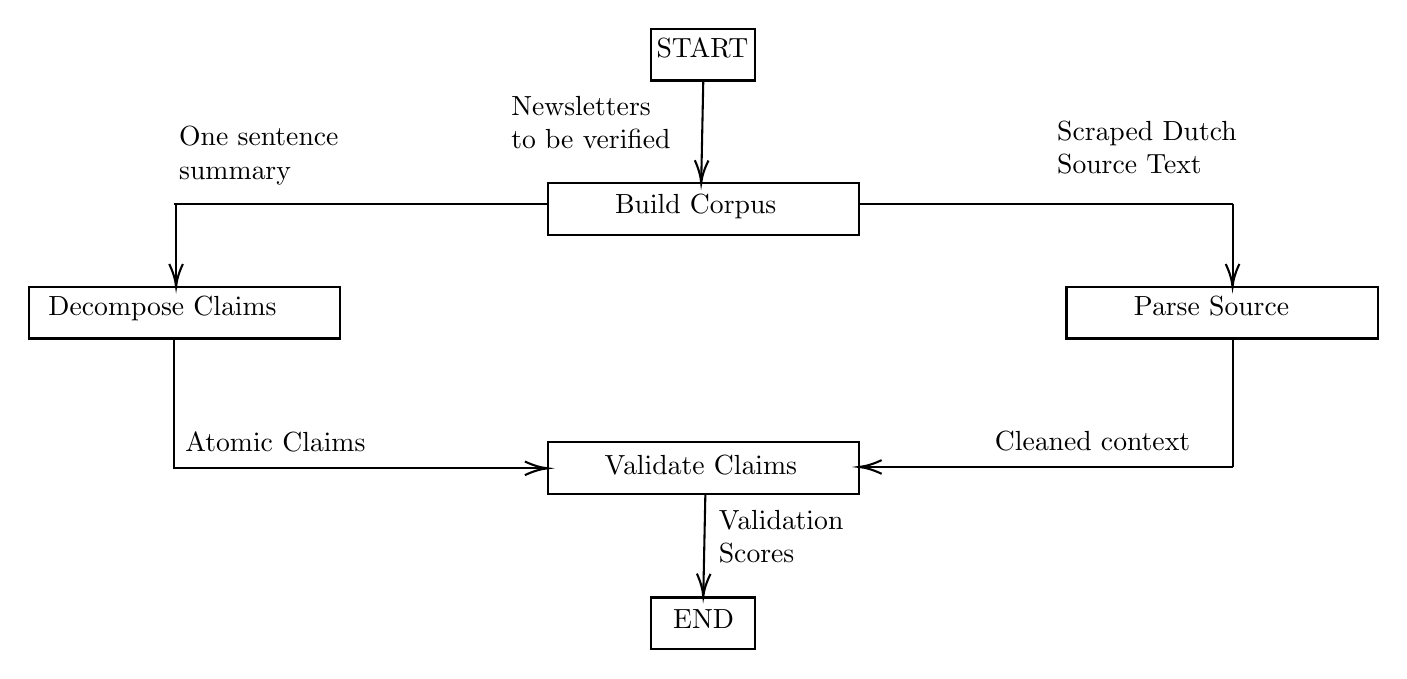
\begin{tikzpicture}[x=0.75pt,y=0.75pt,yscale=-1,xscale=1]
%uncomment if require: \path (0,680); %set diagram left start at 0, and has height of 680

%Shape: Rectangle [id:dp4070963882781028] 
\draw   (300,1) -- (350,1) -- (350,25.96) -- (300,25.96) -- cycle ;
%Shape: Rectangle [id:dp9774405992082825] 
\draw   (250,75.38) -- (400,75.38) -- (400,100.33) -- (250,100.33) -- cycle ;
%Straight Lines [id:da38434376573046714] 
\draw    (325,26.46) -- (324.04,73.38) ;
\draw [shift={(324,75.38)}, rotate = 271.17] [color={rgb, 255:red, 0; green, 0; blue, 0 }  ][line width=0.75]    (10.93,-3.29) .. controls (6.95,-1.4) and (3.31,-0.3) .. (0,0) .. controls (3.31,0.3) and (6.95,1.4) .. (10.93,3.29)   ;
%Shape: Rectangle [id:dp7238715529174791] 
\draw   (0,125.29) -- (150,125.29) -- (150,150.25) -- (0,150.25) -- cycle ;
%Shape: Rectangle [id:dp544713314300144] 
\draw   (500,125.29) -- (650,125.29) -- (650,150.25) -- (500,150.25) -- cycle ;
%Shape: Rectangle [id:dp6187874396247628] 
\draw   (250,200.17) -- (400,200.17) -- (400,225.13) -- (250,225.13) -- cycle ;
%Shape: Rectangle [id:dp9525801403683838] 
\draw   (300,275.04) -- (350,275.04) -- (350,300) -- (300,300) -- cycle ;
%Straight Lines [id:da7731746387458769] 
\draw    (580,85.36) -- (580,123.29) ;
\draw [shift={(580,125.29)}, rotate = 270] [color={rgb, 255:red, 0; green, 0; blue, 0 }  ][line width=0.75]    (10.93,-3.29) .. controls (6.95,-1.4) and (3.31,-0.3) .. (0,0) .. controls (3.31,0.3) and (6.95,1.4) .. (10.93,3.29)   ;
%Straight Lines [id:da8488203549026855] 
\draw    (400,85.36) -- (580,85.36) ;

%Straight Lines [id:da17279727340281192] 
\draw    (580,212.15) -- (402,212.15) ;
\draw [shift={(400,212.15)}, rotate = 360] [color={rgb, 255:red, 0; green, 0; blue, 0 }  ][line width=0.75]    (10.93,-3.29) .. controls (6.95,-1.4) and (3.31,-0.3) .. (0,0) .. controls (3.31,0.3) and (6.95,1.4) .. (10.93,3.29)   ;
%Straight Lines [id:da7845149368668756] 
\draw    (580,150.25) -- (580,212.15) ;

%Straight Lines [id:da8313227318576999] 
\draw    (326,225.62) -- (325.04,272.54) ;
\draw [shift={(325,274.54)}, rotate = 271.17] [color={rgb, 255:red, 0; green, 0; blue, 0 }  ][line width=0.75]    (10.93,-3.29) .. controls (6.95,-1.4) and (3.31,-0.3) .. (0,0) .. controls (3.31,0.3) and (6.95,1.4) .. (10.93,3.29)   ;
%Straight Lines [id:da5767226057733228] 
\draw    (71,85.36) -- (71,123.29) ;
\draw [shift={(71,125.29)}, rotate = 270] [color={rgb, 255:red, 0; green, 0; blue, 0 }  ][line width=0.75]    (10.93,-3.29) .. controls (6.95,-1.4) and (3.31,-0.3) .. (0,0) .. controls (3.31,0.3) and (6.95,1.4) .. (10.93,3.29)   ;
%Straight Lines [id:da09197572758197181] 
\draw    (70,85.36) -- (250,85.36) ;

%Straight Lines [id:da9262340614866109] 
\draw    (70,212.8) -- (248,212.8) ;
\draw [shift={(250,212.8)}, rotate = 180] [color={rgb, 255:red, 0; green, 0; blue, 0 }  ][line width=0.75]    (10.93,-3.29) .. controls (6.95,-1.4) and (3.31,-0.3) .. (0,0) .. controls (3.31,0.3) and (6.95,1.4) .. (10.93,3.29)   ;
%Straight Lines [id:da6502941044352438] 
\draw    (70,213.15) -- (70,150.25) ;


% Text Node
\draw (281,79.11) node [anchor=north west][inner sep=0.75pt]   [align=left] {Build Corpus};
% Text Node
\draw (531,128.52) node [anchor=north west][inner sep=0.75pt]   [align=left] {Parse Source};
% Text Node
\draw (276,204.89) node [anchor=north west][inner sep=0.75pt]   [align=left] {Validate Claims};
% Text Node
\draw (231,31.92) node [anchor=north west][inner sep=0.75pt]   [align=left] {Newsletters \\to be verified};
% Text Node
\draw (494,43.88) node [anchor=north west][inner sep=0.75pt]   [align=left] {Scraped Dutch \\Source Text};
% Text Node
\draw (464,193.41) node [anchor=north west][inner sep=0.75pt]   [align=left] {Cleaned context};
% Text Node
\draw (71,46.87) node [anchor=north west][inner sep=0.75pt]   [align=left] {One sentence \\summary};
% Text Node
\draw (74,193.91) node [anchor=north west][inner sep=0.75pt]   [align=left] {Atomic Claims};
% Text Node
\draw (8,128.52) node [anchor=north west][inner sep=0.75pt]   [align=left] {Decompose Claims};
% Text Node
\draw (331,231.58) node [anchor=north west][inner sep=0.75pt]   [align=left] {Validation \\Scores};
% Text Node
\draw (309,279.27) node [anchor=north west][inner sep=0.75pt]   [align=left] {END};
% Text Node
\draw (301,4.23) node [anchor=north west][inner sep=0.75pt]   [align=left] {START};


\end{tikzpicture}
\caption{System architecture flowchart demonstrating the corpus ingestion, atomic claim decomposition branches, and cross-lingual source verification steps.}
\label{fig:pipeline_flowchart}
\end{figure}
Each paragraph will explain in depth the architectural choices that were made and how each part of the pipeline works. 

\subsection{Dataset and Corpus Construction} \label{rsh:datacorpus}
Before any validation or evaluation is possible, we need to load the source data given in the newsletters url part. This allows us to create a so-called \textit{corpus} which contains all available data we have on the artist we are evaluating.
This corpus is setup as a deterministic and sandboxed evaluation dataset, rather than executing live web scraping and external API queries during the NLI and KG evaluation phases. By doing all the data loading up front, we save time loading all data again when our pipeline crashes later on, or if we wish to run the experiment again. 

This process collects the data in three simple steps: loading the local venue data, fetching the MusicBrainz facts, and saving everything to a JSON file.

\subsubsection{Extracting Venue Data}
As mentioned in Chapter \ref{Newsletter}, our primary data source is a generated newsletter, where we will be focussing on the venue Doornroosje, located in Nijmegen. This is setup using an automated web scraper, where the primary event details and the LLM-generated summaries are manually extracted from these newsletters and provided to the script. 

A comprehensive breakdown of the newsletter generation process, including its structural and visual layout, is discussed later in Chapter \ref{ch:cloudspeakers_pipeline} (The Cloudspeakers Pipeline). For the purpose of constructing this evaluation corpus, the script strictly isolates the English promotional text—which serves as our target for hallucination detection—alongside the core billing metadata required to identify the performing artists.

\subsubsection{Gathering MusicBrainz Knowledge}
Once the primary event data is manually set up, the script automatically fills the dataset with verified real-world facts by querying the MusicBrainz API. To respect the strict rate-limiting policies enforced by the MusicBrainz infrastructure, the script utilizes a mandatory one-second delay between consecutive requests, ensuring the outbound traffic remains at or below $1 request \slash second$. 

For every artist identified in the venue data, the script searches the API to retrieve three specific data points: their geographic origin, associated musical genres, and any registered aliases. This factual data is stored to serve as the ground truth for detecting extrinsic hallucinations later in the pipeline. 

Given that mid-tier venues frequently program niche, emerging, or highly localized artists, it is expected that some acts will be entirely absent from the MusicBrainz database. To ensure the robustness of the dataset generation, the script implements explicit error handling. If an artist cannot be resolved, the pipeline catches the exception and assigns empty values to the factual fields rather than terminating the program, allowing the script to safely proceed to the next entity.


\subsection{Decomposer}\label{rsh:decomposer}
The main task of the decomposer step is to view the claims made by the LLM in the generated summary. A summary can contain from one untill multiple claims, so it is important that all of them get separated into atomic claims and get evaluated. We define a claim as `atomic' if it contains exactly one predicate-argument relationship, which allows the subsequent NLI model to render a definitive Entailment or Contradiction label without semantic noise.

While state-of-the-art frameworks like Google DeepMind's SAFE \cite{safe2024longform} rely on LLM prompting to decompose long-form summaries into atomic claim, introducing yet another machine learning model and creating high operational and computational costs, we made the choice to do this in a deterministic fashion. Our methodology adopts the core multi-stage atomic decomposition paradigm pioneered by SAFE, but replaces the LLM parser with a deterministic, rule-based linguistic dependency parse utilizing \texttt{spaCy}. Splitting claims into atomic claims, has been proven to improve performance in NLI for multiple models \cite{huang2026atomicsnlifinegrainednaturallanguage} and our own small scale testing (See Table \ref) \additions{Add table to show atomic claims give better results (maybe?)}. Our decomposer has been developed in parallel to the framework given by Huang et al. 


Crucially, by utilizing a deterministic linguistic dependency parser rather than a secondary LLM for claim decomposition, we avoid the `recursive hallucination' risk. When an LLM is used to decompose a summary, it may introduce its own hallucinations during the parsing phase. Our rule-based approach ensures that the decomposition remains faithful to the text's syntactic structure, effectively providing a stable, verifiable input for the subsequent NLI evaluation.

The core of our decomposer consists of treating a sentence as a hierarchical Dependency Tree, where words are nodes connected by functional relationships. These relationships mimic the function of words in English sentences, such as a \textit{preposition}, \textit{subject}, \textit{object}. The enumeration below shows the implementation of the algorithm. 
\begin{enumerate}
    \item Convert the raw text into a machine-readable dependency tree. This allows the system to identify the grammatical roles of words, such as which terms function as the subject and which function as the object of an action.
    \item Iterate through every token in the document to locate ``action anchors." The system prioritizes VERB and AUX (auxiliary verbs such as `is' or `has'), as these words define the core events or states necessary for a factual claim.
    \item Resolving Components: 
    \begin{itemize}
        \item Subject: Identify the nominal subject (`nsubj'). If the subject is a pronoun (e.g., ``He"), replace it with the primary entity name to ensure the claim remains contextually independent and verifiable.
        \item Verb Phrase: Collect all auxiliary verbs to preserve the original tense (e.g., ``is performing").
        \item Object: Locate the grammatical receiver of the action (direct object, attribute, or complement).
        \item Modifiers: Identify surrounding phrases that provide extra context, such as time, location, or manner.
    \end{itemize}
    \item  Combine the subject, verb phrase, and object to construct a coherent, standalone sentence that represents the core fact.
    \item If the sentence includes modifiers, ``multiply" the base statement by each modifier to generate individual, independent claims. This step converts one complex sentence into multiple simple, verifiable statements.
    \item  Perform final data hygiene. Remove exact duplicate claims and discard any fragments that are under 5 words in length. This ensures the final output contains only high-quality, meaningful information.
\end{enumerate}

\subsection{Dutch Parser}

\subsection{Validator}
\subsubsection{Theory}
Validating the claims is the core part of the operation we are doing. The validation is a process of cross-language NLI, comparing the original Dutch text to the English summaries that are given. 

% explain why we used RoBERTa over other choices 
To avoid the inherent bias of self-validation—where an LLM acts as an uncritical judge of its own generated output
\footnote{In the Netherlands, this specific conflict of interest is known as acting such as the company `WC-Eend', referencing
 a famous advertising campaign in which the brand recommends its own product (Wij van Wc-Eend adviseren Wc-Eend).}, \changes{move footnote to introduction.}
the option of using a generative model for the entailment check was discarded.
\textcolor{red}{Even though multiple studies have shown this to be effective, 
we wish to find a way to do this in a deterministic way due to LLMs having the nature of being unpredictable and prone to hallucination, 
as mentioned in section \ref{pre:sec:llm}. } 
\source{find the studies that show LLM can verify themselves.}
Comparing the premise and the hypothesis can be done in multiple ways, but for this thesis we have made the choice to make use of Facebook's XLM-RoBERTa \cite{conneau2020unsupervised}. 

XLM-RoBERTa, is a Transformer-based language model trained on 2.5 Terabytes of filtered CommonCrawl data across 100 different languages.
XLM-R learns a shared mathematical representation of human language, which results in it being able to convert multiple languages into a mapped mathematical vector space, meaning different languages can be compared. 
Conneau et al. show that XLM-R is very competitive with strong monolingual models on XNLI benchmarks, demonstrating that it is possible to have a single large model for all languages. \cite{conneau2020unsupervised} For the Cloudspeakers Experiment (section \ref{Newsletter}), this saves us steps from translating between Dutch and English, or limiting the experiments to pages that \textit{do} have an English variant. 
As mentioned in \ref{pre:sec:nli}, NLI looks at the entailment, contradiction and neutral scores. XLM-R outputs these when given a premise and hypothesis and using these we can determine likelihood of a hallucination by the LLM. 

Guidelines to the entailment scores can be found in Table XX. \additions{add table with entailment Guidelines}

\begin{verbatim}
    INSERT TABLE HERE
\end{verbatim}


\subsubsection{Implementation}
The \texttt{validator} is implemented in Python utilizing PyTorch and the HuggingFace \texttt{transformers} library, using the specific \texttt{joeddav/xlm-roberta-large-xnli} model. 

As mentioned in section XX, the pipeline delivers multiple different claims $\mathcal{C}$ and the original text from the source. Since XLM-R is set up to only check one premise against a single hypothesis, we will run the model 
for every claim and every sentence in the source material and find which sentence results in the highest entailment and which in the highest contradiction. We chose to run the experiments in this way, since it showed the best results in testing compared to supplying the model with the entire source text at once. 
For any given claim ($c \in \mathcal{C}$) and a set of source sentences ($\mathcal{S}$), the system iterates through $\mathcal{S}$, tokenizing the premise-hypothesis pairs with trunaction enabled. 
The raw logits output by the model are passed through a Softmax function to calculate a probability distribution across the earliers mentions classes: \texttt{contradiction}, \texttt{neutral} and \texttt{entailment}. The script holds two trackers for each claim:
\begin{enumerate}
    \item \texttt{max\_entailment}: The sentence in $\mathcal{S}$ that returns the highest \textit{entailment} probability
    \item \texttt{max\_contradiction}: The sentence in $\mathcal{S}$ that returns the highest \textit{contradiction} probability.
\end{enumerate}
\optional{Psuedocode for to show the for loops and explain complexity?}
Testing results can be found in Table XX. These tests showed that XLM-R struggles when the premise and hypothesis aren't of the same length, most likely due to too much information being fed and flooding it with information, leading to a more neutral score. 
These results are back up by SOURCE HERE!!! \source{Back up claim that one sentence is better than full text.}
\subsection{Classification} \optional{Classification could be an option}
